\documentclass{article}
\input{template.tex}


\begin{document}

\title{Preliminary knowledge of diffraction and point spread function (PSF)}
\maketitle


\section{Introduction}
Delurring image is a fundamental problem in image processing, which aims to recover a sharp image from a blurred one, especially useful in the microscopy field.
A formal mathematical model of the blurring process is often given by the convolution of the original image with a function called the point spread function (PSF), which describes how a single point of light is spread out in the image, due to the diffraction phenomenon. This function is essential for understanding and correcting the blurring effect, yet it is often unknown in practice. Therefore, estimating the PSF from the blurred image is a crucial step in the deblurring process. A understanding of the physical principles behind the PSF in particular and the diffraction of light in general is necessary to develop effective methods for estimating the PSF. In this report, we will review the basic principles of optics and the diffraction of light, and how they relate to the PSF.

\section{Propagation of light}
Light, as largely accepted, has a dual nature, exhibiting both wave-like and particle-like properties.
In the context of optics and image processing, we often focus on the wave nature of light, which is described by the electromagnetic wave theory.
For the sake of simplicity, we consider only monochromatic light, i.e light that is composed by a single wavelength.
While propagating, light behavior differently according to the environment in which it is propagating.
We focus on the two cases: free-space propagation and propagation through an aperture. The final case is what call diffraction, which will be discussed in~\cref{sec:diffraction}.

Light can be express as a complex-valued function of space and time, consider a point source of light located at a point $P_0$ in space, its complex field at this point can be written as:
\begin{equation}\label{eq:light_field}
E(P_0, t) = A(t) e^{-j2\pi\nu t}
\end{equation}
where $A$ is the amplitude of the wave, $\nu$ is the frequency , $t$ is time.

\paragraph{Free-space} Here we mention "free-space" in a very informal way, without having a rigorous definition.
Intuitively, it means that the light is propagating in a homogeneous medium, i.e the refractive index is constant, without any obstacles or boundaries that could affect its behavior.
Assume that in the space that we are considering, there is only one point source of light located at $P_0$, the complex field at a point $P$ in space can be expressed as:
\begin{equation}\label{eq:free_space}
E(P, t) = \frac{E(P_0, t)}{r} e^{-jkr}
\end{equation}
where $r$ is the distance between the point source and the point $P$, and $k$ is the wave number of the light, which can be expressed as $k = \frac{n 2 \pi \nu}{c}$, where n is the refractive index of the medium. 
In general, the amplitude of the wave decreases as it propagates, and the phase of the wave at point $P$ is delayed with respect to the phase at source point $P_0$ by an amount proportional to the distance $r$.

\paragraph{The intensity of wave field} The intensity of a scalar monochromatic wave at point $P$ is defined as the squared magnitude of the complex phasor representation $U(P)$ of the disturbance:
\begin{equation}
I(P) = |U(P)|^2
\end{equation}

\section{Scalar diffraction theory}\label{sec:diffraction}

\subsection{From a vector to a scalar theory}
When light propagates through an aperture, it can be diffracted, which means that the light waves can bend around the edges of the aperture and interfere with each other, creating a pattern of light and dark regions on a screen placed behind the aperture. The smaller the aperture area, the more significant the diffraction effect.

To understand the diffraction phenomenon, we first state the Maxwell's equations, which describe the behavior of electromagnetic fields, including light. In free space, these equations can be written as:
\begin{align}
\nabla \cdot \epsilon \, \mathbf{E} &= 0 \\
\nabla \cdot \mu \,\mathbf{H} &= 0 \\
\nabla \times \mathbf{E} &= -\mu \,\frac{\partial \mathbf{H}}{\partial t} \\
\nabla \times \mathbf{H} &= \epsilon \,\frac{\partial \mathbf{E}}{\partial t} 
\end{align}
where $\mathbf{E} = (E_x, E_y, E_z)$ is the electric field, $\mathbf{H} = (H_x, H_y, H_z)$ is the magnetic field, $\mu_0$ is the permeability of free space, and $\epsilon_0$ is the permittivity of free space.
The symbol $\times$ and $\cdot$ denote the cross product and dot product, respectively.
$\epsilon$ and $\mu$ are the permittivity and permeability of the environment respectively. More precisely, $\epsilon = \epsilon_r \epsilon_0$ and $\mu = \mu_r \mu_0$, these quantities are related to the refractive index $n$ of the environment and the speed of light $c$ by the following equations:
\begin{equation}\label{eq:refractive_index}
n = \sqrt{\frac{\mu}{\epsilon}}  \qquad \text{and} \qquad c = \frac{1}{\sqrt{\mu \, \epsilon \,}}
\end{equation}

The first two equations state that the divergence of the electric and magnetic fields is zero, which implies the conservation of 
We consider first the following relation:
\begin{equation}
    \nabla \times (\nabla \times \mathbf{E}) = \nabla (\nabla \cdot \mathbf{E}) - \nabla^2 \mathbf{E}
\end{equation} 
The term $\nabla (\nabla \cdot \mathbf{E})$ is zero according to the first Maxwell's equation, while the term $\nabla \times (\nabla \times \mathbf{E})$ can be expressed using the third Maxwell's equation as follows:
\begin{equation}
\nabla \times (\nabla \times \mathbf{E}) = -\mu \frac{\partial}{\partial t} (\nabla \times \mathbf{H}) = -\mu \, \epsilon \, \frac{\partial^2 \mathbf{E}}{\partial t^2}
\end{equation}
Combining the above equations, we can derive the wave equation for the electric field:
\begin{equation}
\nabla^2 \mathbf{E} - \mu \, \epsilon \, \frac{\partial^2 \mathbf{E}}{\partial t^2} = 0
\end{equation}
Or, by using~\cref{eq:refractive_index}, we can express the wave equation as:
\begin{equation}
\nabla^2 \mathbf{E} - \frac{n^2}{c^2} \frac{\partial^2 \mathbf{E}}{\partial t^2} = 0
\end{equation}
The similar wave vector equation can be also derived for the magnetic field $\mathbf{H}$.
Since this wave vector equation is obeyed by each component of the electric field, we can write it arbitrarily for any of the components of $\mathbf{E}$ and $\mathbf{H}$, as a single scalar wave equation:
\begin{equation}\label{eq:scalar_wave_equation}
\nabla^2 U - \frac{n^2}{c^2} U = 0
\end{equation}
Note that this scalar wave equation is an approximation of the full vector wave equation.
It is valid under certain conditions, such as when the light is propagating in a homogeneous medium, where $\epsilon$ and $\mu$ are constant, and there is no obstacle matters in the propagating path of the wave, in such a case, each component of the electric field evolves independently as described by the scalar wave equation. 

In the case of diffraction by an aperture, the fields $\mathbf{E}$ and $\mathbf{H}$ are modified at the edges of the aperture, the scalar wave equation can break in these zones as, the components of electric field become coupled, for example a change in the $E_x$ component can induce a change in the $E_y$ and $E_z$ components, and vice versa. However, if the aperture is large enough compared to the wavelength of the light, the coupling between the components of the electric field can be neglected, and the scalar wave equation can still be used to describe the diffraction phenomenon.

\subsection{Some mathematical Preliminary}
Before embarking on a treatment of diffraction itself, we first consider a number of
mathematical preliminaries that form the basis of the later diffraction theory derivations.

\subsubsection{Green's theorem}
Calculation of the complex field $U$ at an observation point in space can be accomplished by using Green's theorem, that can be stated as follows:
\begin{theorem}
Let $U$ and $G$ be two complex-valued functions of the spatial position, let $S$ be a closed surface surrounding a volume $V$, and let $n$ be the outward normal to the surface $S$. If $U$ and $G$ and their first and second derivatives are single-valued and continuous in $V$ and on $S$, then the following relation holds:
\begin{equation}\label{eq:green_theorem}
\int_V (U \nabla^2 G - G \nabla^2 U) \, dV = \int_S \left( U \frac{\partial G}{\partial n} - G \frac{\partial U}{\partial n} \right) \,dS
\end{equation}
where $\frac{\partial}{\partial n}$ denotes the derivative in the direction of the outward normal to the surface $S$.
\end{theorem}
A careful and strategic choice of an auxiliary function $G$, which we call the Green's function, can allow us to calculate the complex field $U$ at an observation point in space, as we will see in the next section.

\subsection{The integral theorem of Helmholtz and Kirchhoff}
The Kirchhoff formulation of the diffraction problem is based on a certain integral theorem which expresses the solution of the homogeneous wave equation at an arbitrary point in terms of the values of the solution and its first derivative on an arbitrary closed surface surrounding that point.

Let the point of observation be $P_0$, and let $S$ be a closed surface surrounding $P_0$, as indicated in the~\cref{fig:fig35}. Our objective is to calculate the complex field at $P_0$ in terms of its values on $S$. As discussed previously, one should first choose an appropriate Green's function $G$ to be used in the Green's theorem. Kirchhoff's choice of the Green's function is the solution of the inhomogeneous wave equation with a point source at $P_0$, which at a point $P_1$, can be expressed as:
\begin{equation}\label{eq:free_space_green_function}
    G(P1) = \frac{e^{-jk \len{\vect{P_0 P_1}}}}{\len{\vect{P_0 P_1}}}
\end{equation}
where the $\len{.}$ denotes the Euclidean length, and $k$ is the wave number of the light.

The Green's theorem required that the functions $U$ and $G$ (as well as their first and second partial derivatives) must be continuous within the enclosed volume V.
We remarque the $G$ defined in~\cref{eq:free_space_green_function} is not continuous at $P_0$. Therefore, to exclude the discontinuite at $P_0$, a small spherical surface $S_\varepsilon$ of radius $\varepsilon$ is inserted about the point $P_0$.
Green's theorem is then applied on the volume of intergration V' enclosed by the surface $S$ and the small spherical surface $S_\varepsilon$, and the surface of intergration is $S' = S \cup S_\varepsilon$, the union of the two surfaces $S$ and $S_\varepsilon$, as illustrated in~\cref{fig:fig35}. Note that the normal vector is outward from the volume of integration.
\begin{figure}
\centering
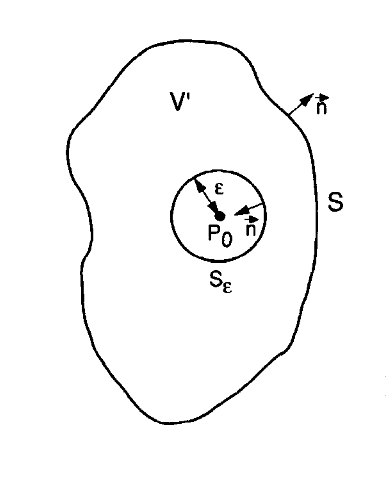
\includegraphics[width=0.5\textwidth]{figures/figure3.5.png}
\caption{\label{fig:fig35}Surface of integration.}
\end{figure}

One may notice that the Green's function $G$ defined in~\cref{eq:free_space_green_function} satisfies the so-called Helmholtz equation (you can verify it using the definition of laplacian operator in spherical coordinates $\nabla^2 G = \frac{1}{r^2} \frac{\partial}{\partial r} \left( r^2 \frac{\partial G}{\partial r} \right)$):
\begin{equation}\label{eq:helmholtz_equation}
(\nabla^2 + k^2) G = 0
\end{equation}

Substituting~\cref{eq:helmholtz_equation} into the left-hand side of~\cref{eq:green_theorem}, we find
\begin{equation}
\int_V (U \nabla^2 G - G \nabla^2 U) \, dV = \int_V (U (-k^2 G) - G (-k^2 U)) \, dV = 0
\end{equation}

Thus the theorem reduces to:
\begin{equation}\label{eq:integral_theorem}
\int_{S \cup S_\varepsilon} \left( U \frac{\partial G}{\partial n} - G \frac{\partial U}{\partial n} \right) \,dS = 0
\end{equation} 

\begin{equation}\label{eq:integral_over_union_surface}
    \int_{S} \left( U \frac{\partial G}{\partial n} - G \frac{\partial U}{\partial n} \right) \,dS + \int_{S_\varepsilon} \left( U \frac{\partial G}{\partial n} - G \frac{\partial U}{\partial n} \right) \,dS = 0
\end{equation}

We first calculate the second term of the above equation, which is the integral over the small spherical surface $S_\varepsilon$. One has:
\begin{align}
    \frac{\partial G}{\partial n} &= \frac{\partial G}{\partial r} \, \vect{n_\varepsilon} \\
    &= \frac{e^{jk \len{\vect{P_0 P_1}}}}{\len{\vect{P_0 P_1}}^2}  \left(jk - \frac{1}{\len{\vect{P_0 P_1}}}\right) \vect{P_0 P_1} \cdot \vect{n_\varepsilon} 
\end{align}
For a point $P_1$ on the small spherical surface $S_\varepsilon$, we have  $\vect{P_0 P_1} \cdot \vect{n_\varepsilon} = 1$ and $\len{\vect{P_0 P_1}} = \varepsilon$, thus we can express $\frac{\partial G}{\partial n}$ as:
\begin{equation}
    \frac{\partial G}{\partial n} = -\frac{e^{jk \varepsilon}}{\varepsilon^2}  \left(jk - \frac{1}{\varepsilon}\right)
\end{equation}
Let $\varepsilon$ become arbitrarily small:
\begin{equation}
\lim_{\varepsilon \to 0} \int_{S_\varepsilon} \left( U \frac{\partial G}{\partial n} - G \frac{\partial U}{\partial n} \right) \,dS =
\lim_{\varepsilon \to 0} 4 \pi  \left[U(P_0) \, e^{jk \varepsilon}  \left(jk - \frac{1}{\varepsilon}\right) - \frac{\partial U(P_0) \, e^{jk \varepsilon} \,\varepsilon}{\partial n} \right] = -4 \pi U(P_0)
\end{equation}
Substituting the above result into~\cref{eq:integral_over_union_surface}, we can express the complex field at the observation point $P_0$ as:
\begin{equation}\label{eq:Helmholtz_Kirchhoff}
U(P_0) = \frac{1}{4 \pi} \int_{S} \left( U \frac{\partial G}{\partial n} - G \frac{\partial U}{\partial n} \right) \,dS
\end{equation}
This is the integral theorem of Helmholtz and Kirchhoff, which allows to express the complex field at an arbitrary point in terms of the values of the solution and its first derivative on an arbitrary closed surface surrounding that point.

\subsection{The diffraction formula by a planar screen}
\subsubsection{Application of the integral theorem}
We are now in a position to apply the integral theorem of Helmholtz and Kirchhoff to the problem of diffraction by an aperture in an infinite opaque screen.

As shown in the~\cref{fig:fig36}, a wave disturbance is assumed to impinge on the screen and the aperture from the left, and the field at the point $P_0$ behind the aperture is to be calculated. Following Kirchhoff, the closed surface $S$ is chosen to consist of two parts: the surface $S_1$ lying directly behind the diffracting screen, to be joined and closed by a large spherical cap $S_2$ of radius $R$ centered at the observation point $P_0$. The total closed surface $S$ is then the union of $S_1$ and $S_2$.
\begin{figure}
\centering
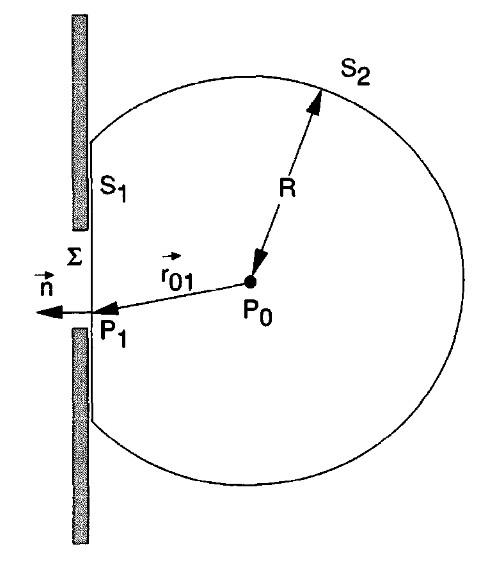
\includegraphics[width=0.5\textwidth]{figures/figure3.6.png}
\caption{\label{fig:fig36}Diffraction of light by an aperture in an infinite opaque screen.} 
\end{figure}

On $S_2$, the green function $G$ reduce to:
\begin{equation}
G = \frac{e^{-jkR}}{R}
\end{equation}
and its normal derivative can be expressed as:
\begin{equation}
\frac{\partial G}{\partial n} = \frac{e^{-jkR}}{R^2}  \left(jk - \frac{1}{R}\right) \approx jkG
\end{equation}

The approximation is valid when the radius $R$ of the spherical cap $S_2$ is large enough compared to the wavelength $\lambda$, in such a case, the term $\frac{1}{R}$ can be neglected compared to the term $jk = j \, \frac{2\pi}{\lambda}$.

The integral over the surface $S_2$ can be expressed as:
\begin{align}
\int_{S_2} \left( U \frac{\partial G}{\partial n} - G \frac{\partial U}{\partial n} \right) \,dS &= \int_\Omega \left( U \frac{\partial G}{\partial n} - G \frac{\partial U}{\partial n} \right) R^2 d\omega \\
&= \int_\Omega G \left( jkU - \frac{\partial U}{\partial n} \right) R^2 d\omega
\end{align}
where $\Omega$ is the solid angle subtended by the surface $S_2$ at the observation point $P_0$.

We notice that the quantity $RG = e^{-jkR}$ is bounded on $S_2$. Moreover, there is a very convenient condition that allow us to dispose this above integral, this condition is called the \textit{Sommerfeld radiation condition}, which states that the field $U$ must vanishes at least at fast as a diverging spherical:
\begin{equation}\label{eq:sommerfeld_condition}
\lim_{R \to \infty} R \left( \frac{\partial U}{\partial R} - jkU \right) = 0
\end{equation}
This condition guarantees that we are dealing only with outgoing waves on $S_2$, rather than incoming waves, for which the condition is not satisfied. By using the Sommerfeld radiation condition, the integral over the surface $S_2$ will yield a contribution of zero.


There is an another reasonning for the zero contribution of the integral over the surface $S_2$, which as $R$ becomes surficially large, the field $U$ have not existed on  $S_2$, as the wave is travaled with a finite speed, therefore, the field $U$ and its normal derivative $\frac{\partial U}{\partial n}$ will be zero on $S_2$, thus the integral over the surface $S_2$ will also yield a contribution of zero.

\subsubsection{The Kirchhoff boundary conditions}
Having disposed of the integral over the surface $S_2$, we are left with the integral over the surface $S_1$:
\begin{equation}\label{eq:integral_over_S1}
    U(P_0) = \frac{1}{4 \pi} \int_{S_1} \left( U \frac{\partial G}{\partial n} - G \frac{\partial U}{\partial n} \right) \,dS
\end{equation}

The screen is opaque, except for the open aperture which will be denoted by $\Sigma$. It is therefore seems Intuitively that the major contribution to the integral over $S_1$ will come from the open aperture $\Sigma$, and the contribution from the opaque part of the screen will be negligible. This is the basis of the Kirchhoff boundary conditions, which state that:
\begin{itemize}
    \item Accross the surface $\Sigma$, the field $U$ and its normal derivative $\frac{\partial U}{\partial n}$ are equal to the values they would have if the screen were not present.
    \item Over the portion of the surface $S_1$ that is occupied by the opaque screen, the field $U$ and its normal derivative $\frac{\partial U}{\partial n}$ are zero.
\end{itemize}
By using the Kirchhoff boundary conditions, the \cref{eq:integral_over_S1} can be expressed as:
\begin{equation}\label{eq:integral_over_aperture}
    U(P_0) = \frac{1}{4 \pi} \int_{\Sigma} \left( U \frac{\partial G}{\partial n} - G \frac{\partial U}{\partial n} \right) \,dS
\end{equation}
While the Kirchhoff boundary conditions reduces the problem's complexity, the conditions are only valid for the aperture whose dimensions are large compared to the wavelength of the light, in this case the obtained results agree very well with experiment.

\subsubsection{The Fresnel-Kirchhoff diffraction formula}
Let write down the normal derivative of the Green's function $G$ at a point $P_1$ on the aperture $\Sigma$:
\begin{equation}
\frac{\partial G}{\partial n}(P_1)  = \frac{e^{-jk \len{\vect{P_0 P_1}}}}{\len{\vect{P_0 P_1}}^2}  \left(jk - \frac{1}{\len{\vect{P_0 P_1}}}\right) \vect{P_0 P_1} \cdot \vect{n} 
\end{equation}

Since $k >> \frac{1}{\len{\vect{P_0 P_1}}}$, we can neglect the term $\frac{1}{\len{\vect{P_0 P_1}}}$ compared to the term $jk$, leading to the following approximation:
\begin{align}
\frac{\partial G}{\partial n} (P_1) &\approx \frac{e^{-jk \len{\vect{P_0 P_1}}}}{\len{\vect{P_0 P_1}}^2}  jk \vect{P_0 P_1} \cdot \vect{n} \\
&= jk \, \frac{e^{-jk \len{\vect{P_0 P_1}}}}{\len{\vect{P_0 P_1}}} \, \cos(\vect{P_0 P_1}, \vect{n})
\end{align}

Now suppose that the aperture is illuminated by a single spherical wave (see~\cref{fig:fig37}), arising from a point source at $P_2$
\begin{equation}
U(P_1) = \frac{A\, e^{jk\len{\vect{P_2 P_1}}}}{\len{\vect{P_2 P_1}}} 
\end{equation}

\begin{figure}
\centering
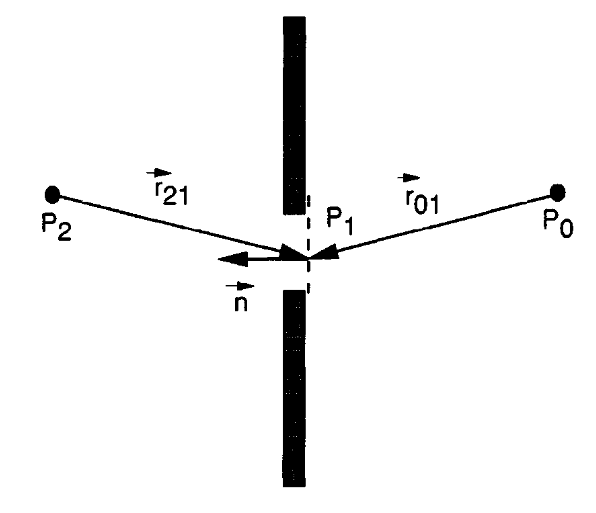
\includegraphics[width=0.5\textwidth]{figures/figure3.7.png}
\caption{\label{fig:fig37} Point-source illumination of a plan screen.}
\end{figure}

If $\len{\vect{P_2 P_1}}$ is large compared to the wavelength, we can make the following approximation on the normal derivative of $U$:
\begin{equation}
\frac{\partial U}{\partial n} (P_1) \approx jk \, \frac{e^{jk\len{\vect{P_2 P_1}}}}{\len{\vect{P_2 P_1}}} \, \cos(\vect{P_2 P_1}, \vect{n})
\end{equation}
Then, \cref{eq:integral_over_aperture} is:
\begin{align}\label{eq:fresnel_kirchhoff_diffraction_formula}
    U(P_0) &= \frac{1}{4\pi} \int_\Sigma \frac{A j k e^{jk\Bigl(\len{\vect{P_2 P_1}}+\len{\vect{P_0 P_1}}\Bigl)}}{\len{\vect{P_2 P_1}} \, \len{\vect{P_0 P_1}}}\, \left( \cos(\vect{P_2 P_1}, \vect{n}) - \cos(\vect{P_0 P_1}, \vect{n})\right) \, dS \\
    &= \frac{1}{2j\lambda}\int_\Sigma \frac{e^{jk\Bigl(\len{\vect{P_2 P_1}}+\len{\vect{P_0 P_1}}\Bigl)}}{\len{\vect{P_2 P_1}} \, \len{\vect{P_0 P_1}}} \left( \cos(\vect{P_0 P_1}, \vect{n}) - \cos(\vect{P_2 P_1}, \vect{n})\right) \, dS
\end{align}
This result, which holds only for an illumination consisting a single point source, is known as the \textit{Fresnel-Kirchhoff diffraction formula}. One can also remark that the formula is symmetric in the source and observation points, thus a point source at $P_0$ will produce the same field at $P_2$ as a point source at $P_2$ will produce at $P_0$. This result is referred to the \textit{reciprocity theorem of Helmholtz}.

We can also rewrite the Fresnel-Kirchhoff diffraction formula in the way that the disturbance at the observation point $P_0$ is expressed as a superposition of the contributions from each point $P_1$ on the aperture $\Sigma$, as follows:
\begin{equation}
U(P_0) = \int_\Sigma U_s(P_1) \, \frac{e^{jk\len{\vect{P_0 P_1}}}}{\len{\vect{P_0 P_1}}} \, dS
\end{equation}
where 
\begin{equation}
U_s(P_1) = \frac{1}{2j\lambda} \, \frac{A e^{jk\len{\vect{P_2 P_1}}}}{\len{\vect{P_2 P_1}}} \, \left( \cos(\vect{P_0 P_1}, \vect{n}) - \cos(\vect{P_2 P_1}, \vect{n})\right)
\end{equation}

\subsection{General diffraction formula} While the Fresnel-Kirchhoff theory has been found experimentally to yield remarkably accurate results and is widely used in practices, there are certain internal inconsistencies. The difficulties of the Kirchhoff theory stem from the fact that boundary conditions must be imposed on both the field strength and its normal derivative. In particular, it is a well-known theorem of potential theory that if a two-dimensional potential function and its normal derivative vanish together along any finite curve segment, then the potential function must vanish over the entire plane. Similarly, if a three-dimensional potential function and its normal derivative vanish together on any finite surface patch, then the potential function must vanish over the entire space. Thus the two Kirchhoff boundary conditions together imply that the field is zero everywhere behind the aperture, a result which contradicts the known physical situation. 

These inconsistencies have motivated a search for a more satisfactory mathematical development, we can name here the Rayleigh-Sommerfeld theory, which is based on a alternative choice of the Green's function, that eliminated the necessity of imposing boundary values on both the disturbance and its normal derivative simultaneously. However, we would not go into the details of the Rayleigh-Sommerfeld theory, but we just state the final result, which is not much different from the Fresnel-Kirchhoff diffraction formula, and is given by:
\begin{equation}
U_I(P_0) = \frac{A}{j\lambda}\int_\Sigma \frac{e^{jk\Bigl(\len{\vect{P_2 P_1}}+\len{\vect{P_0 P_1}}\Bigl)}}{\len{\vect{P_2 P_1}} \, \len{\vect{P_0 P_1}}}  \, \cos(\vect{P_0 P_1}, \vect{n})  \, dS
\end{equation}
\begin{equation}
U_{II}(P_0) = \frac{A}{j\lambda}\int_\Sigma \frac{e^{jk\Bigl(\len{\vect{P_2 P_1}}+\len{\vect{P_0 P_1}}\Bigl)}}{\len{\vect{P_2 P_1}} \, \len{\vect{P_0 P_1}}}  \, \cos(\vect{P_2 P_1}, \vect{n})  \, dS
\end{equation}
The fact that the two above formulas are different is not surprising, as they are based on different choices of the Green's function, and thus they are not expected to yield the same results.

One may notice that the Fresnel-Kirchhoff diffraction formula is the average of the two Rayleigh-Sommerfeld diffraction formulas.
Several experiments have been conducted to compare the predictions of the Fresnel-Kirchhoff and Rayleigh-Sommerfeld theories, and it has been found that these theories yield the same results provided that the aperture dimensions are large compared to the wavelength. In general the two theories can be put in common by introducing a obliquity factor $\psi$, for all case we can write:
\begin{equation}
U(P_0) = \frac{A}{j\lambda}\int_\Sigma \frac{e^{jk\Bigl(\len{\vect{P_2 P_1}}+\len{\vect{P_0 P_1}}\Bigl)}}{\len{\vect{P_2 P_1}} \, \len{\vect{P_0 P_1}}} \, \psi \, dS
\end{equation}
where
\begin{equation}
\psi = \begin{cases}
\frac{1}{2} \left(\cos(\vect{P_0 P_1}, \vect{n}) - \cos(\vect{P_2 P_1}, \vect{n})\right) & \text{Fresnel-Kirchhoff theory} \\
\cos(\vect{P_0 P_1}, \vect{n}) & \text{Rayleigh-Sommerfeld theory I} \\
\cos(\vect{P_2 P_1}, \vect{n}) & \text{Rayleigh-Sommerfeld theory II}
\end{cases}
\end{equation}

for the special case of an infinitely distant point source producing normally incident plane wave illumination, the obliquity factor $\psi$ becomes:
\begin{equation}
\psi = \begin{cases}
\frac{1}{2} \left(1 + \cos(\theta)\right) & \text{Fresnel-Kirchhoff theory} \\
\cos(\theta) & \text{Rayleigh-Sommerfeld theory I} \\
1 & \text{Rayleigh-Sommerfeld theory II}
\end{cases}
\end{equation}
where $\theta$ is the angle formed by $\vect{n}$ and $\vect{P_0 P_1}$.

When only small angles are involved in the diffraction problem, it is easy to
show that all three solutions are identical.
In all three cases the obliquity factors approach unity as the angles become small, and the differences between the results vanish.
Note that only small angles will be involved if we are far from the diffracting aperture.

In closing it is worth noting that, in spite of its internal inconsistencies, there
is one sense in which the Kirchhoff theory is more general than the Rayleigh-Sommerfeld theory.
The latter requires that the diffracting screens be planar, while the former does not.
However, most of the problems of interest here will involve planar diffracting apertures, so this generality will not be particularly significant.
In fact, we will generally choose to use the first Rayleigh-Sommerfeld solution because of its simplicity.

\subsubsection{Fresnel-Fraunhofer diffraction formula}
This section introduces a series of approximations that allow to express the diffraction formula in a more simple form. We first show the coordinate system in which we will express the diffraction formula, as illustrated in~\cref{fig:fig41}.
\begin{figure}
\centering
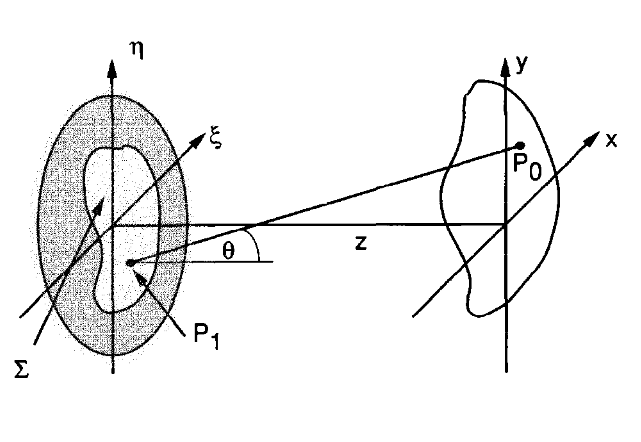
\includegraphics[width=0.5\textwidth]{figures/figure4.1.png}
\caption{\label{fig:fig41}Diffraction geometry.}
\end{figure}


According to \cref{eq:free_space} we can rewrite the general diffraction formula as
\begin{equation}
    U(P_0) = \frac{1}{j\lambda}\int_\Sigma U(P_1) \frac{e^{jk\len{\vect{P_0P_1}}}}{\len{\vect{P_0P_1}}} \, \cos\theta \, dS
\end{equation}
The term $\cos \theta$ is given by:
\begin{equation}
    \cos \theta = \frac{z}{\len{\vect{P_0P_1}}}
\end{equation}

Therefore, the diffraction formula can be rewritten:
\begin{equation}
    U(P_0) = \frac{z}{j\lambda}\int_\Sigma U(P_1) \frac{e^{jk\len{\vect{P_0P_1}}}}{\len{\vect{P_0P_1}}^2} \, dS
\end{equation}

Handling the ecludian distance $\len{\vect{P_0P_1}}$ in the above formula is not an easy task, especially when it is involved in the exponent, we therefore simplify the distance by using the binomial expansion of the square root, stated as follows:
\begin{equation}
    \sqrt{1 + x} = 1 + \frac{1}{2} x - \frac{1}{8} x^2 + \cdots
\end{equation}

Applying the binomial expansion to the distance $\len{\vect{P_0P_1}}$, one gets:
\begin{equation}
    \len{\vect{P_0P_1}} = z \sqrt{1 + \frac{(x-x_1)^2 + (y-y_1)^2}{z^2}} \approx z + \frac{(x-x_1)^2 + (y-y_1)^2}{2z}
\end{equation}
Note that we keep only the first two terms of the binomial expansion, which should be sufficient in the case where the distance $z$ is large compared to $(x-\xi)$ and $(y-\eta)$, which is the case of interest here.
For the term $\len{\vect{P_0P_1}}$ in the denominator, we can also simplify further by using $\len{\vect{P_0P_1}} \approx z$, but this approximation is not valid for one in the nominator as it is involved in the exponent, where even a small error can lead to a significant change in the result. The resulting expression for the complex field at $(x,y)$ therefore becomes:
\begin{equation}\label{eq:fresnel_integral}
    U(x,y) = \frac{e^{jkz}}{j\lambda z}\int_\Sigma U(\xi,\eta) e^{j\frac{k}{2z}\left((x-\xi)^2 + (y-\eta)^2\right)} \,d\xi d\eta
\end{equation}
This formula is known as the \textit{Fresnel integral}

\paragraph{Accuracy of the Fresnel approximation} A strict condition for the validity of the Fresnel approximation must satisfy the following conditinon:
\begin{equation}
    z^3 \gg \frac{k}{8} \left[(x-\xi)^2 + (y-\eta)^2\right]_{max}^2
\end{equation}
For a circular aperture of radius 1cm, a circular observation region of size 1cm, and a wavelength of 0.5$\mu m$, this condition would require that the distance z must be  $\gg$ 25cm for ensureing the accuracy. However, this condition is overstringent, and accuracy can be expected for much shorter distances. It is found that the majority of the contribution to the convolution integral comes from a square in the $(\xi,\eta)$ plane, with width $4\sqrt{z \lambda}$, centered on the point $(\xi=x,\eta=y)$. this square grows in size as the distance $z$ increases. \todo{add more arguments, for instance the condition for that the approximation is valide is not quite clear}

\subsection{Point spread function (PSF) of optical systems}
The most important component of optical imaging and data processing systems are lenses. A lens is composed of an optically dense material, usualy glass with a refractive index $n > 1$, in which the propagation velocity of light is less than the velocity in air.
 In this section, we will derive the point spread function (PSF) of a lens.
\subsubsection{A thin lens as a phase transformation}
A lens is said to be a thin lens if a ray entering at coordinate $(x,y)$ on one face exits at approximately the same coordinate on the other face, i.e if there is negligible translation of a ray within the lens.


Referring to the~\cref{fig:fig51}, let the maximal thickness of the lens (on its axis) be $
\Delta_0$, and let the thickness at coordinatate $(x,y)$ be $\Delta(x,y)$.
According to the free-space propagation formula~\cref{eq:free_space}, the total phase delay of a ray passing through the lens at coordinate $(x,y)$ is given by: 
\begin{equation}
    \phi(x,y) = k \, n \, \Delta(x,y) + k \, (\Delta_0 - \Delta(x,y))
\end{equation}
where n is the refractive index of the lens material, $kn\Delta(x,y)$ is the phase delay introduced by the lens, and $k(\Delta_0 - \Delta(x,y))$ is the phase delay introduced by the remaining region of free space between the two planes.Equivalently, the lens may be represented by a multiplicative phase transformation of the form:
\begin{equation}\label{eq:phase_delay_lens}
    t(x,y) =  e^{j \, k \, \Delta_0} \,e^{j \, k \, (n-1) \, \Delta(x,y)}
\end{equation}

The complex field $U_l'(x,y)$ across the the exit plane immediately behind the lens is then related to the complex field $U_l(x,y)$ across the entrance plane immediately in front of the lens by:
\begin{equation}
    U_l'(x,y) = t(x,y) \, U_l(x,y)
\end{equation}
The problem remains to find the mathematical form of the theckness function $\Delta(x,y)$ in order that the effects of the lens may be understood.

\subsubsection{The thickness function}
In order to specify the forms of the phase transformations introduced by a variety of different types of lenses, we first adopt a sign convention: as rays travel from left to right, each convex surface encountered is taken to have a positive radius of curvature, while each concave surface is taken to have a negative radius of curvature. Thus in~\cref{fig:fig51}, the radius of curvature of the left-hand surface of the lens is a positive number $R_1$, while the radius of curvature of the right-hand surface is a negative number $R_2$.
\begin{figure}
\centering
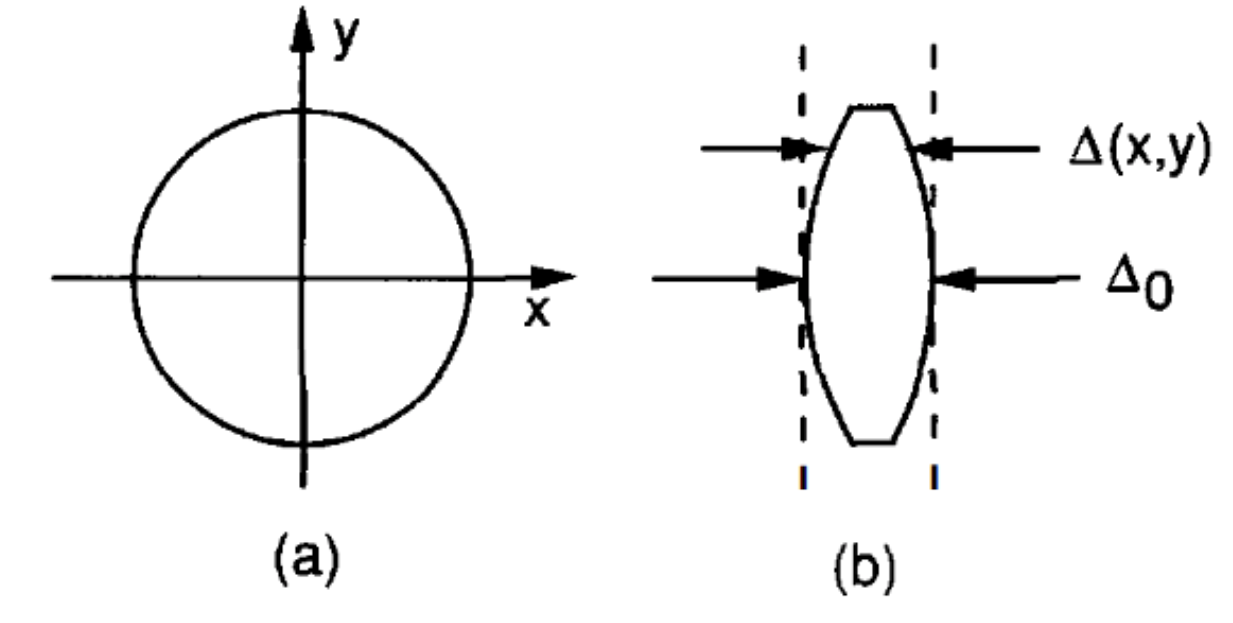
\includegraphics[width=0.5\textwidth]{figures/figure5.1.png}
\caption{\label{fig:fig51}The thickness function: (a) front view, (b) side view.}
\end{figure}

To find the thickness function $\Delta(x,y)$, we split the lens into three regions: the left region $\Delta_1(x,y)$, the middle region $\Delta_2(x,y)$, and the right region $\Delta_3(x,y)$, as illustrated in~\cref{fig:fig52}. the thickness function $\Delta(x,y)$ can then be expressed as:
\begin{equation}
    \Delta(x,y) = \Delta_1(x,y) + \Delta_2(x,y) + \Delta_3(x,y)
\end{equation}
where $\Delta_1(x,y)$, $\Delta_2(x,y)$, and $\Delta_3(x,y)$ are given derived from the geometry of the lens as follows:
\begin{align}
\Delta_1(x,y) &= \Delta_{01} - (R_1 - \sqrt{R_1^2 - (x^2 + y^2)}) \\
&= \Delta_{01} - R_1\left(1 - \sqrt{1 - \frac{x^2 + y^2}{R_1^2}}\right) 
\end{align}
\begin{align}
\Delta_3(x,y) &= \Delta_{03} - (-R_2 - \sqrt{R_2^2 - (x^2 + y^2)}) \\
&= \Delta_{03} + R_2\left(1 - \sqrt{1 - \frac{x^2 + y^2}{R_2^2}}\right) 
\end{align}
The second region $\Delta_2(x,y)$ is a constant. Therefore, the total thickness is seen to be:
\begin{equation}
\Delta(x,y) = \Delta_{0} 
- R_1\left(1 - \sqrt{1 - \frac{x^2 + y^2}{R_1^2}}\right)
+ R_2\left(1 - \sqrt{1 - \frac{x^2 + y^2}{R_2^2}}\right) 
\end{equation}

\begin{figure}
\centering
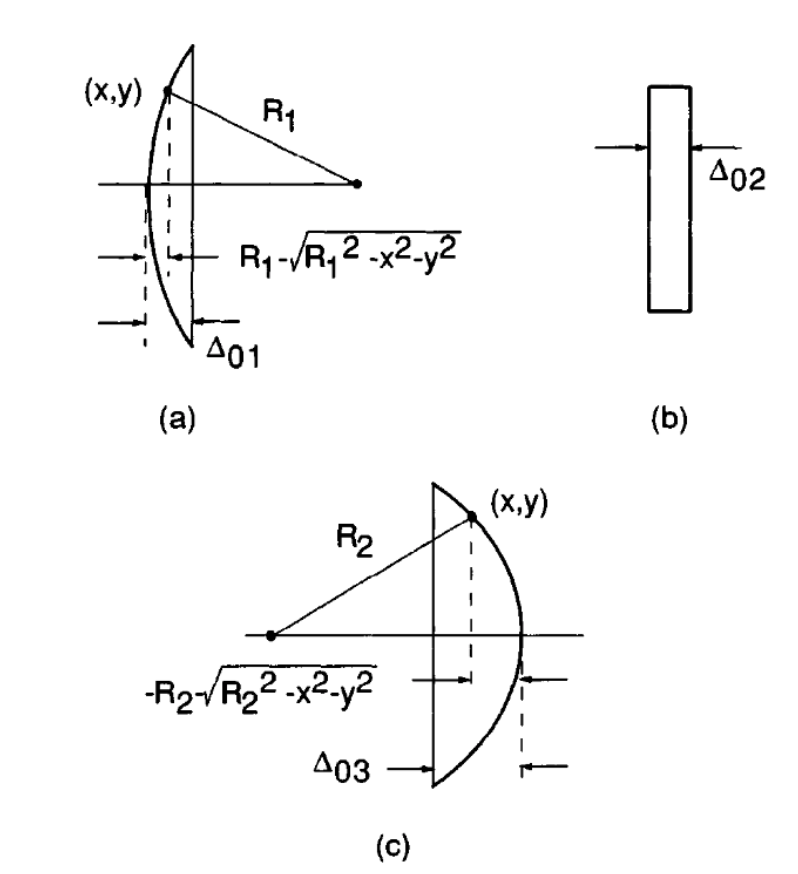
\includegraphics[width=0.5\textwidth]{figures/figure5.2.png}
\caption{\label{fig:fig52}Calculation of the thickness function: (a) geometry for $\Delta_1(x,y)$, (b) geometry for $\Delta_2(x,y)$, (c) geometry for $\Delta_3(x,y)$.}
\end{figure}

The expression of the thickness function $\Delta(x,y)$ can be safely simplified if attention is restricted to the region of the lens near the lens axis, or equivalently, if only paraxial rays are considered. Thus we consider only values of $x$ and $y$ sufficiently small to allow the following approximation to be accurate:
\begin{align}
\sqrt{1 - \frac{x^2 + y^2}{R_1^2}} &\approx 1 - \frac{x^2 + y^2}{2R_1^2} \\
\sqrt{1 - \frac{x^2 + y^2}{R_2^2}} &\approx 1 - \frac{x^2 + y^2}{2R_2^2} \\
\Delta(x,y) &\approx \Delta_0 - \frac{x^2 + y^2}{2} \left( \frac{1}{R_1} - \frac{1}{R_2} \right)
\end{align}

With the help of these approximations, the thickness function becomes:
\begin{equation}\label{eq:total_thickness}
    \Delta(x,y) \approx \Delta_0 - \frac{x^2 + y^2}{2} \left( \frac{1}{R_1} - \frac{1}{R_2} \right)
\end{equation}

\subsubsection{The phase transformation by lenses}
Substituting~\cref{eq:total_thickness} into~\cref{eq:phase_delay_lens} yields the following expression for the phase transformation introduced by the lens:
\begin{equation}
    t(x,y) = e^{j \, k \, \Delta_0} \, e^{j \, k \, (n-1) \, \left( \Delta_0 - \frac{x^2 + y^2}{2} \left( \frac{1}{R_1} - \frac{1}{R_2} \right) \right)}
\end{equation}\

The physical properties of the lens (that is n, $R_1$, and $R_2$) can be combined into a single number f called the \textbf{focal length}, which is defined by:
\begin{equation}\label{eq:focal_length}
    \frac{1}{f} = (n-1) \left( \frac{1}{R_1} - \frac{1}{R_2} \right)
\end{equation}
When f is positive, the lens is called a converging lens or positive lens, then spherical wave is converging toward a point on the lens axis a distance \textbf{f} behind the lens.
 
Neglecting the constant phase factor, which we shall drop hereafter, the phase transformation may now be rewritten
\begin{equation}\label{eq:phase_delay_lens_simple}
    t_l(x,y) = e^{-j \, \frac{k}{2f} \, (x^2 + y^2)}
\end{equation}
This equation will serve as our basic representation of the effects of a thin lens on an incident disturance. Since in our derivation, we did not consider the sign of $R_1$ and $R_2$, the focal length $f$ is therefore general to be applied to any type of lens, as long as the sign convention for the radius of curvature is respected. 

\subsubsection{Fourier transforming property of lenses}
One of the most important properties of converging lenses is that they can perform two-dimensional Fourier transformation on the incident disturbance. This complicated analog operation can be performed with exextreme simplicity in an optical system, taking advantage of the basic laws of propagation and diffraction of light.


\paragraph{Back focal plane} The back focal plane of a converging lens is the plane normal to the lens axis and located at a distance f behind the lens, where f is the focal length of the lens.
\paragraph{Input transparencies} The input transparency is a thin planar object placed in front of the lens, capable of modulating the amplitude and/or phase of the incident light. 

\begin{figure}
\centering
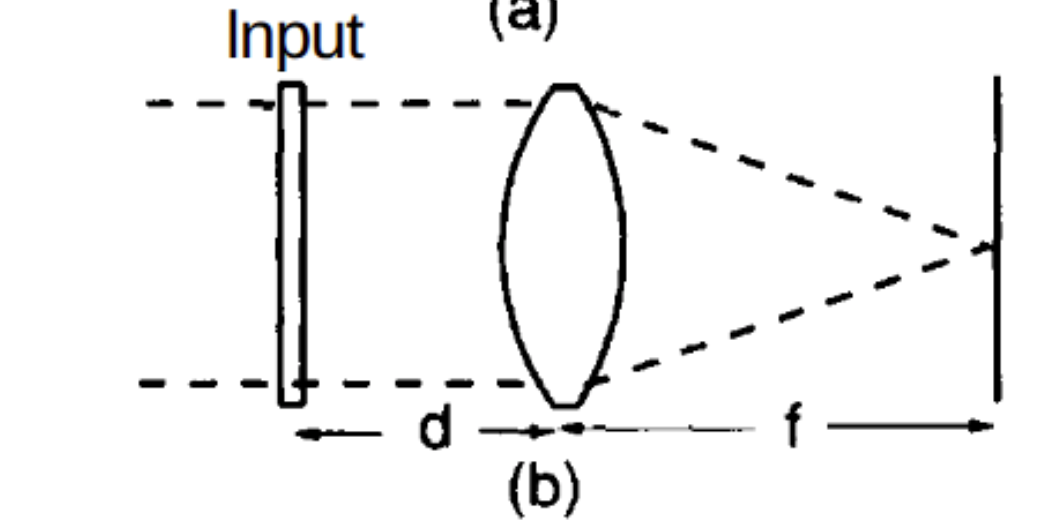
\includegraphics[width=0.5\textwidth]{figures/figure5.5.png}
\caption{\label{fig:fig55}Geometries for perfoming the Fourier transform operator with a converging lens.}
\end{figure}

Figure \ref{fig:fig55} illustrates the arrangement that will be considered here, the input is placed a distance d in front of the lens, is illuminated by a normally incident plane wave of amplitude $A$, and the input transmittance is denoted by $t_A(x,y)$. Let $F_o(f_X, f_Y)$ represent the Fourier spectrum of the light transmitted by the input transparency, and $F_l(f_X, f_Y)$ the Fourier spectrum of the light incident on the lens,
\begin{equation}
    F_o(f_X, f_Y) = \mathcal{F}(A \, t_A(x,y)) \quad \quad F_l(f_X, f_Y) = \mathcal{F}(U_l(x,y))
\end{equation}
where $U_l(x,y)$ is the complex field across the entrance plane of the lens which,according to the fresnel integral~\cref{eq:fresnel_integral}, can be expressed as:
\begin{align}
    U_l(x,y) &= \frac{e^{jkd}}{j\lambda d}\int_\Sigma A \, t_A(\xi,\eta) e^{j\frac{k}{2d}\left((x-\xi)^2 + (y-\eta)^2\right)} \,d\xi d\eta\\
    &= \left((A\, t_A) \ast h\right) (x,y)
\end{align}
where $h(x,y) = \frac{e^{jkd}}{j\lambda d} e^{j\frac{k}{2d}(x^2 + y^2)}$ 

We can now express the Fourier spectrum of the light incident on the lens as follows:
\begin{align}
    F_l(f_X, f_Y) &= \mathcal{F}(U_l(x,y)) \\
    &= \mathcal{F}\left( \left((A\, t_A) \ast h\right) (x,y) \right) \\
    &= F_o(f_X, f_Y) \cdot H(f_X, f_Y)
\end{align}
where $H(f_X, f_Y) = \mathcal{F}(h)(f_X, f_Y)$ is the Fourier spectrum of the impulse response $h(x,y)$, which can be calculated as follows:
\begin{align}
    H(f_X, f_Y) &= \mathcal{F}(h)(f_X, f_Y) \\
    &= \frac{e^{jkd}}{j\lambda d} \int_{-\infty}^{\infty} \int_{-\infty}^{\infty} e^{j\frac{k}{2d}(x^2 + y^2)} e^{-j2\pi(f_X x + f_Y y)} \, dx dy \\
    &= \frac{e^{jkd}}{j\lambda d} \int_{-\infty}^{\infty} e^{j\frac{k}{2d}x^2} e^{-j2\pi f_X x} \, dx \int_{-\infty}^{\infty} e^{j\frac{k}{2d}y^2} e^{-j2\pi f_Y y} \, dy \\
    &= \frac{e^{jkd}}{j\lambda d} e^{-j \pi \lambda d (f_X^2)} e^{-j \pi \lambda d (f_Y^2)} \\
    &= \frac{e^{jkd}}{j\lambda d} e^{-j \pi \lambda d (f_X^2 + f_Y^2)}
\end{align}

The finite extent of the lens can be accounted for by associating with the lens a pupil function $P(x,y)$ defined by:
\begin{equation}
    P(x,y) = \begin{cases}
1 & \text{if } (x,y) \text{ is within the lens aperture} \\
0 & \text{otherwise}
\end{cases}
\end{equation}

Thus the amplitude distribution behind the lens can be expressed as:
\begin{align}
    U_l'(x,y) &= U_l(x,y) P(x,y) t_l(x,y) \\
    &= U_l(x,y) P(x,y) e^{-j \, \frac{k}{2f} \, (x^2 + y^2)}
\end{align}

To find the distribution U



\end{document}